
\documentclass[12pt]{article}
\usepackage[hungarian]{babel}
\selectlanguage{hungarian}
\usepackage[utf8]{inputenc}
\usepackage[T1]{fontenc}

\pdfpageheight\paperheight
\pdfpagewidth\paperwidth
\setlength\topmargin{-7mm} \setlength\oddsidemargin{-0cm}
\setlength\textheight{22cm} \setlength\textwidth{15.8cm}
\setlength\columnsep{0.25in}  \newlength\titlebox \setlength\titlebox{2.00in}
\setlength\headheight{5pt}   \setlength\headsep{0pt}
\setlength\footskip{1.9cm}
\setlength\leftmargin{0.0in}

\usepackage{alltt}

\usepackage{tikz}
\usetikzlibrary{shapes,shapes.geometric,shapes.multipart,calc}
\tikzset{
  data/.style={
      draw,
      rectangle split,
      rectangle split parts=2,
      text centered,
  },
  data+/.style={
      data,
      rectangle split every empty part={},
      rectangle split empty part width=\widthof{#1},
      rectangle split empty part height=\heightof{#1},
      rectangle split empty part depth=\depthof{#1}
  }
}
\usepackage{wasysym}
\date{}
\title{2. gyakorlat -- Kibővített keresőfák}
\begin{document}

\maketitle

\noindent1. Tekintsük az alábbi bináris keresőfát rendezettminta-faként!\\
Emlékeztető: a rendezettminta-fa olyan bináris keresőfa, amely minden $p$ gyökerű részfára eltárolja azt a kiegészítőinformációt, hogy hány elemet tartalmaz a $p$ gyökerű részfa.

\begin{figure}[!h]
\centering
  \begin{tikzpicture}[level/.style={sibling distance = 9cm/#1},level distance = 1.cm]
    \node[data]{
\includegraphics[height=1cm]{kenguru.png} \nodepart{two} }
        child{ node[data]{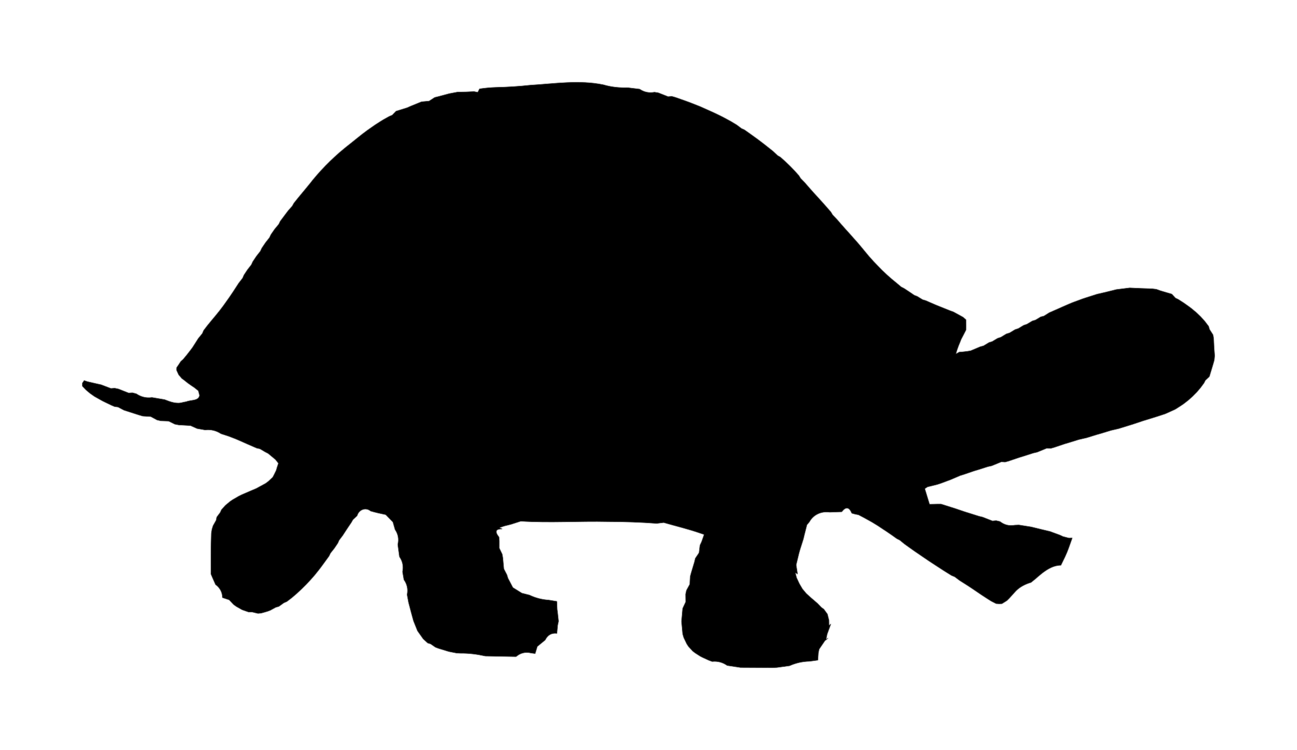
\includegraphics[height=0.75cm]{turtle.png} \nodepart{two}}
    	    child{ node[data]{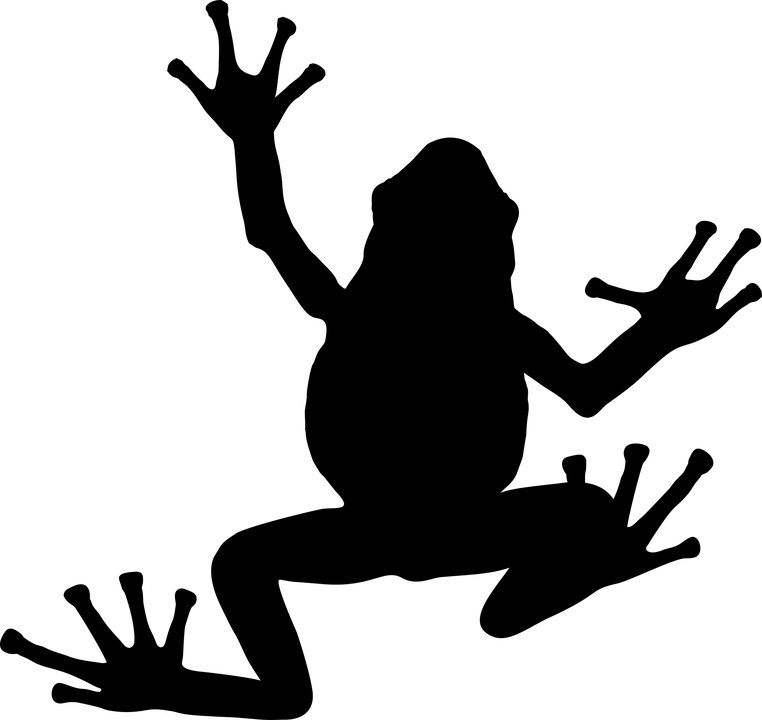
\includegraphics[height=0.75cm]{frog.png} \nodepart{two}}}
            child{ node[data]{
\includegraphics[height=0.75cm]{wolf.jpg} \nodepart{two}}
                child{ node[data]{
\includegraphics[height=0.75cm]{ozike.jpg} \nodepart{two}}
                       child{ node[data]{
\includegraphics[height=0.75cm]{hare.jpg} \nodepart{two}}}
                       child[missing]                    
                }
                child{ node[data]{
\includegraphics[height=0.75cm]{delphin.jpg} \nodepart{two}}}
            }
        }
        child{ node[data]{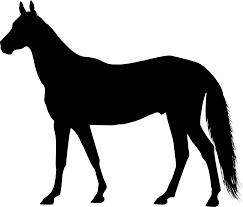
\includegraphics[height=0.75cm]{horse.png} \nodepart{two}}
            child{ node[data]{
\includegraphics[height=0.75cm]{lion.jpg} \nodepart{two}}}
            child{ node[data]{
\includegraphics[height=0.75cm]{giraffe.jpg} \nodepart{two}}
                child{ node[data]{
\includegraphics[height=0.75cm]{bear.jpg} \nodepart{two}}}
                child[missing]
            }
        };
  \end{tikzpicture}
\end{figure}

\noindent a) Határozzuk meg a fában lévő kulcsok $<$ reláció szerinti rendezését!

\noindent b) Töltsük ki a rendezettminta-fából hiányzó kiegészítő információkat!\\
Milyen fabejárással lehetne kitölteni a fából hiányzó, rendezettminta-fák által használt kiegészítő információkat? \\
Megjegyzés: a valóságban persze nem ''utólag'', fabejárást használva határozzuk meg a kiegészítőinformációkat, hanem a műveletek végrehajtása során aktualizáljuk azokat!

\noindent c) A kiegészítő információkra támaszkodva adjuk meg a $<$ rendezés szerinti

\begin{itemize}
\item 6 rangú elemet
\begin{alltt}
RangKeres(
\includegraphics[height=0.4cm]{kenguru.png}, 6)
RangKeres(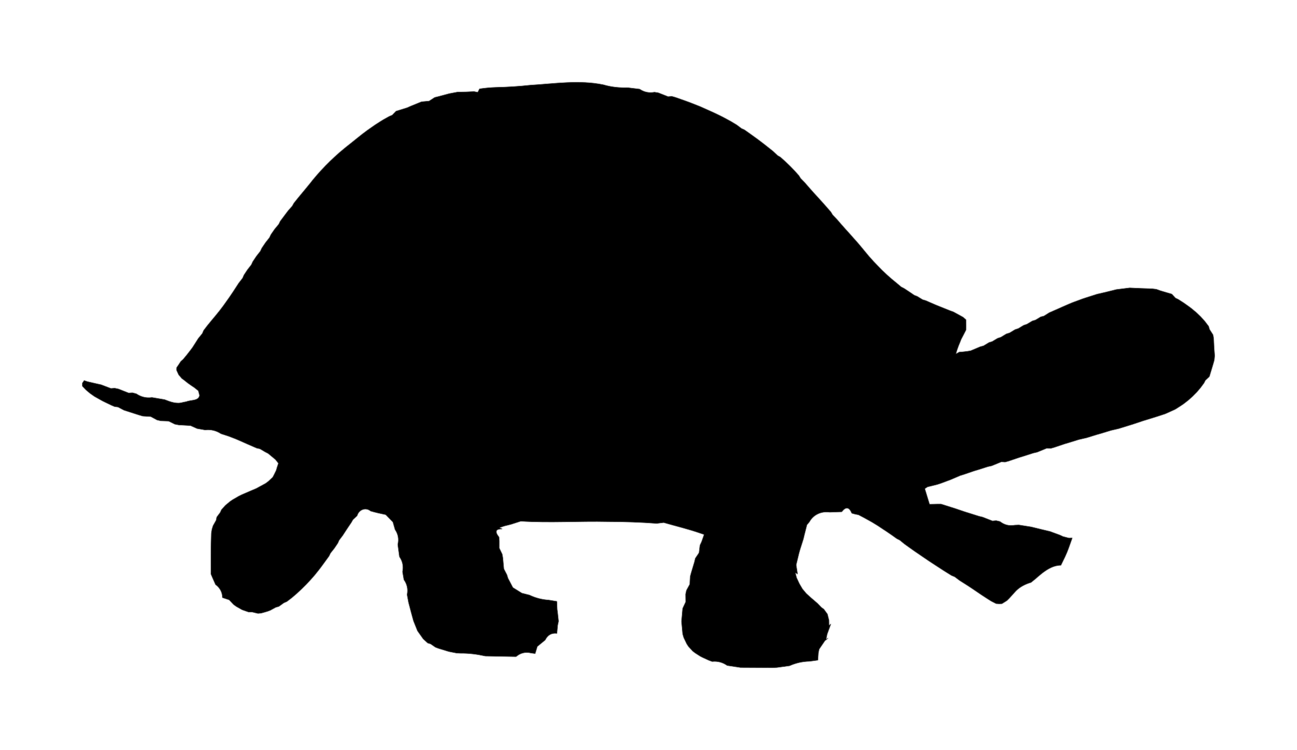
\includegraphics[height=0.4cm]{turtle.png}, 6)
RangKeres(
\includegraphics[height=0.4cm]{wolf.jpg}, 4)
RangKeres(
\includegraphics[height=0.4cm]{delphin.jpg}, 1)
\end{alltt}

\item 9 rangú elemet
\begin{alltt}
RangKeres(
\includegraphics[height=0.4cm]{kenguru.png}, 9)
RangKeres(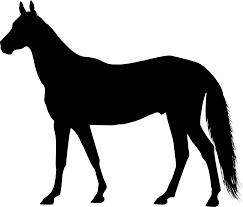
\includegraphics[height=0.4cm]{horse.png}, 2)
\end{alltt}
\end{itemize}

\noindent d) A kiegészítő információk alapján mi lesz $
\includegraphics[height=0.4cm]{wolf.jpg}$ rangja?\\
Megjegyzés: $r_{x}(
\includegraphics[height=0.4cm]{wolf.jpg})$ az $
\includegraphics[height=0.4cm]{wolf.jpg}$ szimbólum rangjára vonatkozó aktuális ismereteinket jelöli abban a pillanatban, amikor az algoritmus az $x$ jelű csúcs feldolgozásánál tart. \\
$r_{
\includegraphics[height=0.4cm]{wolf.jpg}}(
\includegraphics[height=0.4cm]{wolf.jpg})=1+2$\\
$r_{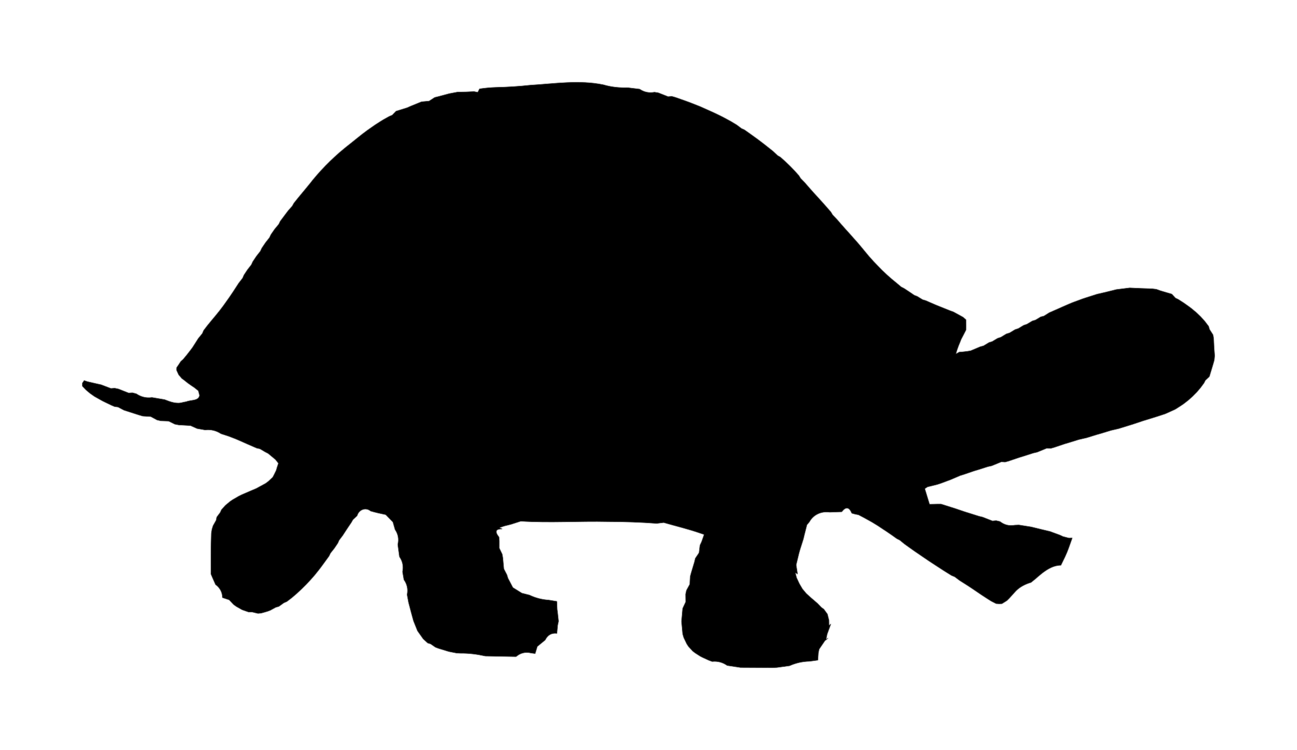
\includegraphics[height=0.4cm]{turtle.png}}(
\includegraphics[height=0.4cm]{wolf.jpg})=r_{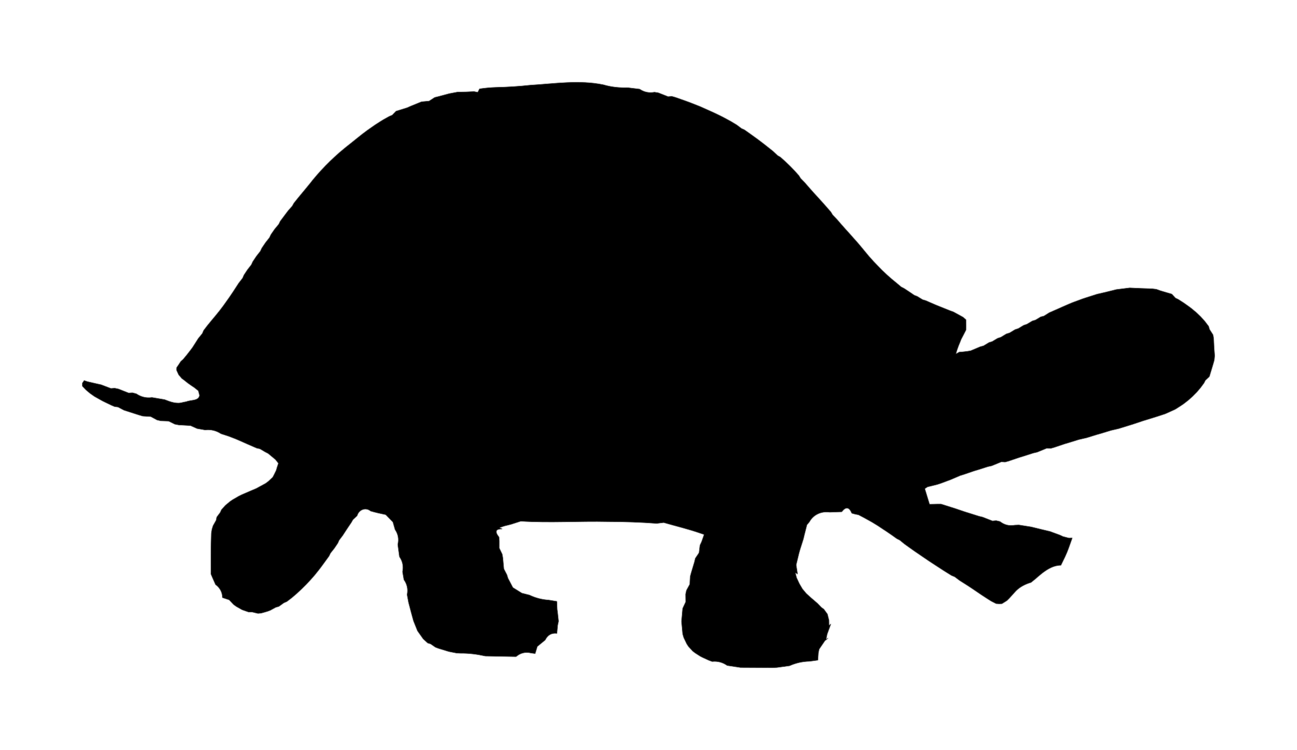
\includegraphics[height=0.4cm]{turtle.png}}(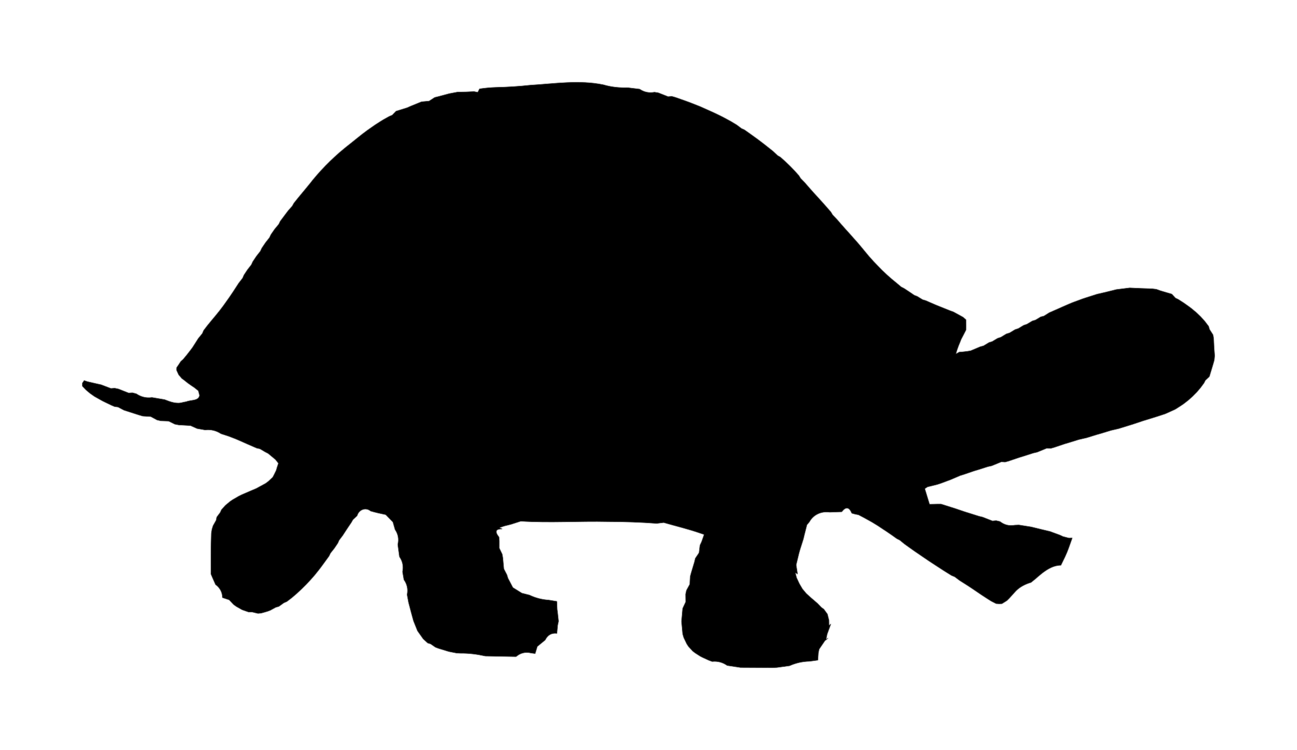
\includegraphics[height=0.4cm]{turtle.png})+1+1$\\
$r_{
\includegraphics[height=0.4cm]{kenguru.png}}(
\includegraphics[height=0.4cm]{wolf.jpg})=r_{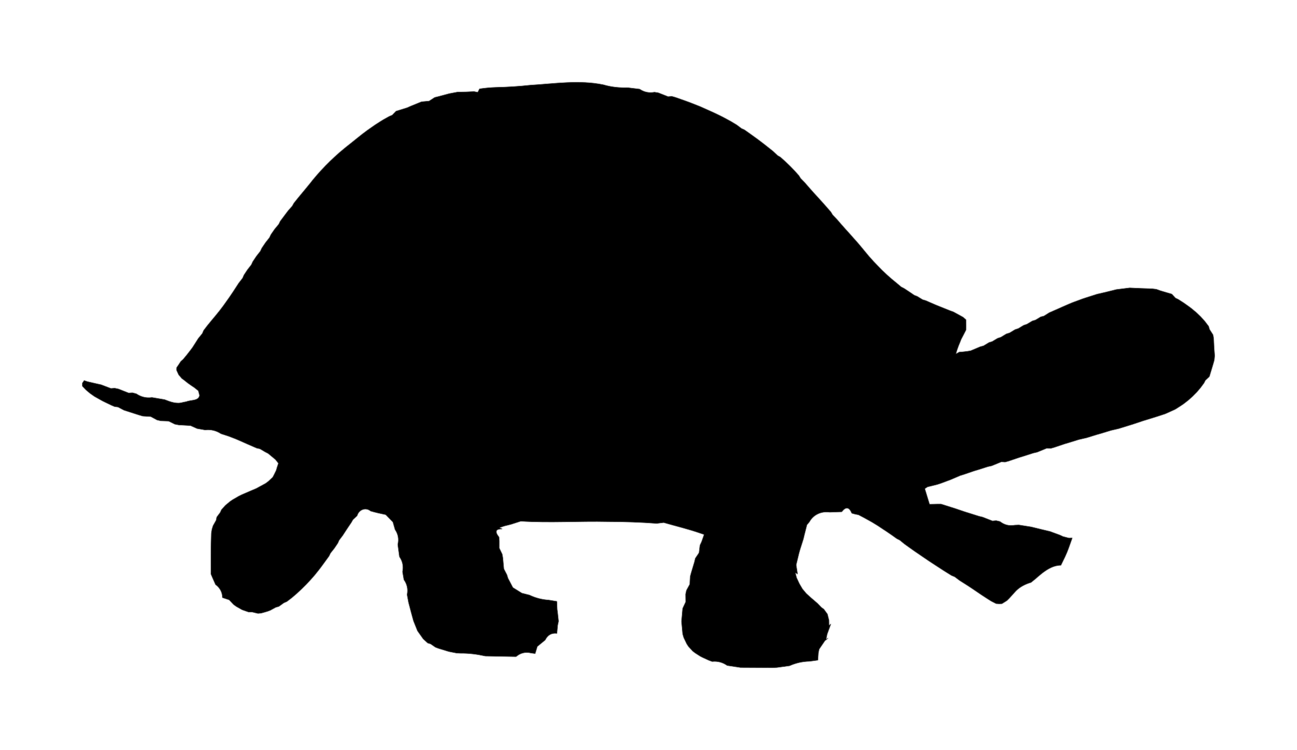
\includegraphics[height=0.4cm]{turtle.png}}(
\includegraphics[height=0.4cm]{wolf.jpg})+0=5$\\

\noindent e) Hajstuk végre a {\scshape Beszúr(
\includegraphics[height=0.4cm]{rhinoceros.png})}, illetve a {\scshape Töröl(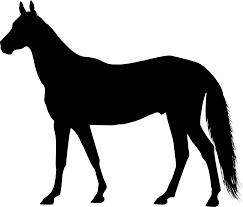
\includegraphics[height=0.4cm]{horse.png})} műveleteket, amennyiben tudjuk, hogy a $
\includegraphics[height=0.4cm]{rhinoceros.png} < 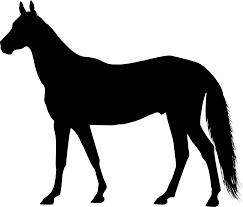
\includegraphics[height=0.4cm]{horse.png}$, illetve a $
\includegraphics[height=0.4cm]{rhinoceros.png} > 
\includegraphics[height=0.4cm]{lion.jpg}$ relációk teljesülnek!



\begin{figure}[!h]
\centering
  \begin{tikzpicture}[level/.style={sibling distance = 8cm/#1},level distance = .9cm]
    \node[data]{
\includegraphics[height=1cm]{kenguru.png} \nodepart{two}11 }
        child{ node[data]{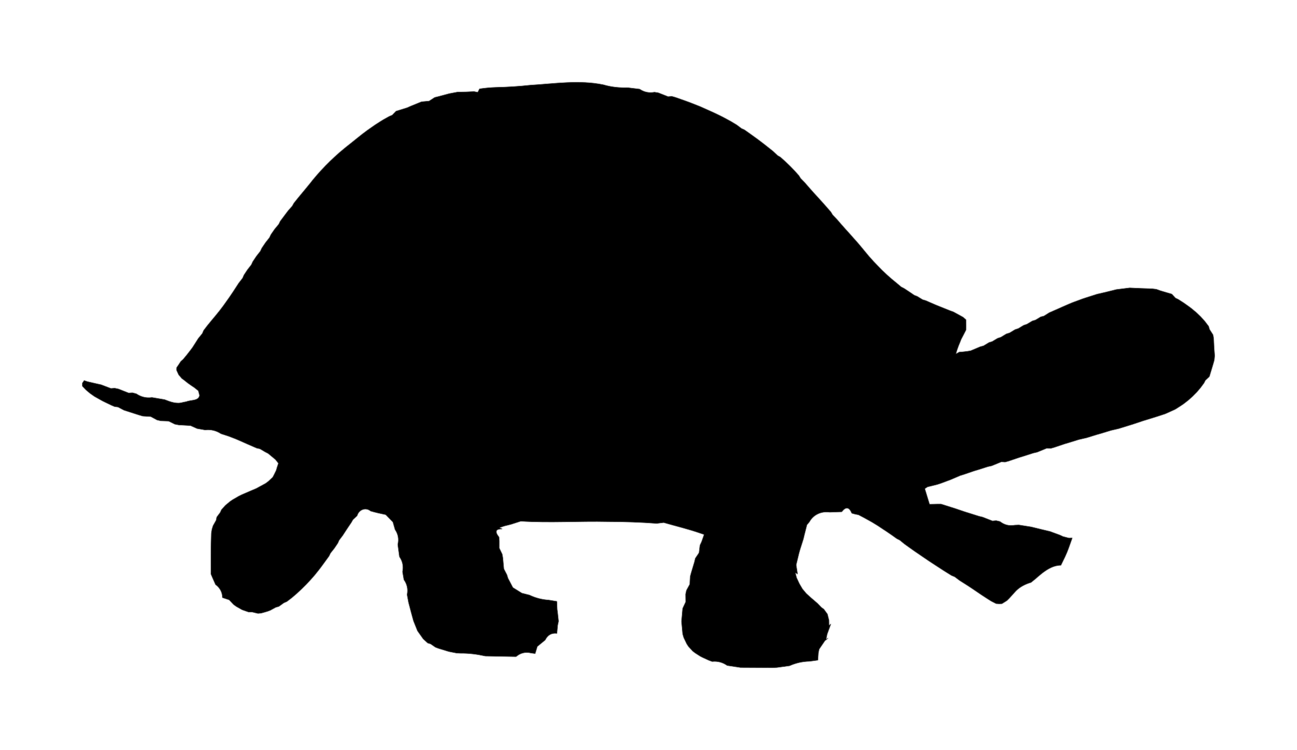
\includegraphics[height=0.75cm]{turtle.png} \nodepart{two}6}
    	    child{ node[data]{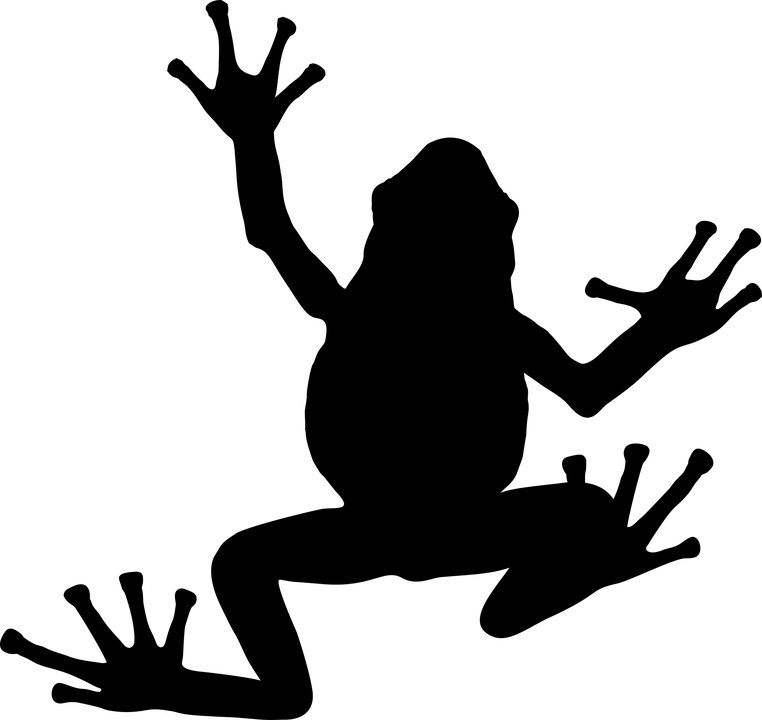
\includegraphics[height=0.75cm]{frog.png} \nodepart{two}1}}
            child{ node[data]{
\includegraphics[height=0.75cm]{wolf.jpg} \nodepart{two}4}
                child{ node[data]{
\includegraphics[height=0.75cm]{ozike.jpg} \nodepart{two}2}
                       child{ node[data]{
\includegraphics[height=0.75cm]{hare.jpg} \nodepart{two}1}}
                       child[missing]                    
                }
                child{ node[data]{
\includegraphics[height=0.75cm]{delphin.jpg} \nodepart{two}1}}
            }
        }
        child{ node[data]{
\includegraphics[height=0.4cm]{rhinoceros.png} \nodepart{two}4}
            child{ node[data]{
\includegraphics[height=0.75cm]{lion.jpg} \nodepart{two}1}}
            child{ node[data]{
\includegraphics[height=0.75cm]{giraffe.jpg} \nodepart{two}2}
                child{ node[data]{
\includegraphics[height=0.75cm]{bear.jpg} \nodepart{two}1}}
                child[missing]
            }
        };
  \end{tikzpicture}
\end{figure}

\noindent 2. Szúrjuk be az alábbi intervallumokat egy kezdetben üres intervallum-fába: \\
$[16;21], [8;9], [5;8], [25;30], [15;23], [17;19],
[26;26], [0;3], [6;10]$.\\
A beszúrásnál bal végpont a kulcs. $p$ csúcs kiegészítő információja a $p$ gyökerű részfában lévő intervallumok jobb végpontjainak maximuma.
{\scshape Beszúrás/Törlés} során a kiegészítő információkat -- a rendezettminta-fához hasonlóan -- aktualizálnunk kell.

\begin{figure}[!h]
\centering
    \begin{tikzpicture}[level/.style={sibling distance = 9cm/#1},level distance = 1.6cm]
    \node[data]{[16;21]\nodepart{two}30}
        child{
            node[data]{[8;9]\nodepart{two}23}
            child{node[data] {[5;8]\nodepart{two}10}
               child{node[data]{[0;3]\nodepart{two}3}}
               child{node[data]{[6;10]\nodepart{two}10}}
            }
            child{node[data] {[15;23]\nodepart{two}23}}
            }
        child{
            node[data]{[25;30]\nodepart{two}30}
            child{node[data]{[17;19]\nodepart{two}19}}
            child{node[data]{[26;26]\nodepart{two}26}}
        };
    \end{tikzpicture}
\end{figure}

\noindent Keresés a gyökérből indul és amíg nem talál fedő intervallumot addig nézi, hogy a keresett intervallum
bal végpontja $\leq$ az aktuális csúcs bal fiának kiegészítő információja, akkor balra megy a fában, egyébként
jobbra.

\noindent {\scshape ÁtfedőKeres([22;25])}: $[16;21] \rightarrow [8;9] \rightarrow \mathbf{[15;23]} \rightarrow \smiley$ \\
{\scshape ÁtfedőKeres([11;14])}: $[16;21] \rightarrow [8;9] \rightarrow [15;23] \rightarrow \frownie$

\end{document}
